\documentclass[10pt]{beamer}
 
\usepackage{macros-beamer}

\usepackage[utf8]{inputenc}

\usepackage{tikz-cd}

\usetikzlibrary{decorations.pathmorphing}
\usetikzlibrary{decorations.markings}
\tikzset{
	% >=stealth', %%  Uncomment for more conventional arrows
    vector/.style={decorate, decoration={snake}, draw},
	provector/.style={decorate, decoration={snake,amplitude=2.5pt}, draw},
	antivector/.style={decorate, decoration={snake,amplitude=-2.5pt}, draw},
    fermion/.style={draw=black, postaction={decorate},
        decoration={markings,mark=at position .55 with {\arrow[draw=black]{>}}}},
    fermionbar/.style={draw=black, postaction={decorate},
        decoration={markings,mark=at position .55 with {\arrow[draw=black]{<}}}},
    fermionnoarrow/.style={draw=black},
    gluon/.style={decorate, draw=black,
        decoration={coil,amplitude=4pt, segment length=5pt}},
    scalar/.style={dashed,draw=black, postaction={decorate},
        decoration={markings,mark=at position .55 with {\arrow[draw=black]{>}}}},
    scalarbar/.style={dashed,draw=black, postaction={decorate},
        dwecoration={markings,mark=at position .55 with {\arrow[draw=black]{<}}}},
    scalarnoarrow/.style={dashed,draw=black},
    electron/.style={draw=black, postaction={decorate},
        decoration={markings,mark=at position .55 with {\arrow[draw=black]{>}}}},
	bigvector/.style={decorate, decoration={snake,amplitude=4pt}, draw},
}

\newcommand{\vin}{\rotatebox[origin=c]{-90}{$\in$}}
 
 \setbeamertemplate{footline}[frame number]
 
%Information to be included in the title page:
\title{The holomorphic $\sigma$-model and its symmetries}
\author{Brian Williams}
\institute{Northwestern University \\ Advisors: John Francis and Kevin Costello}
\date{May 1, 2018}

\begin{document}

\frame{\titlepage}

\begin{frame}
\frametitle{Outline of this talk}
\begin{enumerate}
\item Rapid overview of the Batalin-Vilkovisky (BV) formalism.
\item Holomorphic theories, in general. 
One-loop finiteness and a formula for the general chiral anomaly. 
\item The holomorphic $\sigma$-model and its factorization algebra.
\end{enumerate}
\end{frame}

\begin{frame}[fragile]
\frametitle{The BV formalism}
The BV formalism is a technique used to study quantizations of field theories.
A generalization of the usual problem of {\em deformation quantization}.
\ben
\begin{tikzcd}
{\rm SympMfld} \arrow[r, "\sO"] & {\rm Alg}_{\rm Poiss} & {\rm Alg}_{\CC[[\hbar]]} \arrow[l,"\hbar \to 0"'] \\
(M, \omega) \arrow[r, mapsto] & \left(\sO(M), \Pi_\omega\right) & \left(\sO(M)[[\hbar]], \star\right) \arrow[l, mapsto] . 
\end{tikzcd}
\een

In field theory, one works on a smooth manifold $X$ (the spacetime). 
\ben
\begin{tikzcd}
{\rm BV-Theory}(X) \ar[r, "{\rm Obs}"] & {\rm FactAlg} (X)_{P_0} & {\rm FactAlg}(X)_{{\rm BV}} \ar[l,"\hbar \to 0"'] .
\end{tikzcd}
\een
Given a classical BV theory we study lifts of the $P_0$ factorization algebra of classical observables to the $BV$ factorization algebra of quantum observables.

In the one-dimensional case $X = \RR$ there exists a classical BV theory associated to a symplectic manifold $(M, \omega)$. 
In this case, BV quantization recovers ordinary deformation quantization. 
\end{frame}

\begin{frame}
\frametitle{The BV formalism (cont.)}
In QFT, BV algebras provide a mathematical model for the path integral (see Costello's book on renormalization). 
\begin{dfn}
A BV algebra is a triple $(A, Q, \Delta)$ where $(A, Q)$ is a commutative dg algebra, and $\Delta : A \to A$ is a degee one linear map such that
\begin{enumerate}[(a)] 
\item $\Delta^2 = [\Delta, Q] = 0$;
\item the degree one bilinear map
\ben
\{a,b\} := \Delta(ab) - \Delta(a) b \pm a \Delta(b)
\een
satisfies graded Jacobi, and is a graded biderivation with respect to the commutative product. 
\end{enumerate}
\end{dfn}
Thus $\{-,-\}$ behaves like a Poisson bracket, except with a weird shift. 
We say an element $I = I_0 + \hbar I_1 + \cdots \in A[[\hbar]]$ satisfies the {\em quantum master equation} (QME) if
\ben
\boxed{(Q+ \hbar \Delta) e^{I/\hbar} = 0 .}
\een
We call $\hbar$ the {\em perturbation} parameter. 
\end{frame}

\begin{frame}
\frametitle{The BV formalism (cont.)}
When we set $\hbar = 0$, the QME reduces to condition
\ben
\boxed{Q I_0 + \frac{1}{2} \{I_0,I_0\} = 0}.
\een
We call this the classical master equation (CME).
\begin{eg}
Suppose $A = \sO(V) = \Sym(V^*)$ for some graded vector space $V$. 
Then a functional $I_0$ satisfying the CME is equivalent to an data of an $L_\infty$ structure on the graded vector space $V[-1]$. 
\end{eg}
Most important example of BV algebras in QFT come from $(-1)$-shifted geometry.
Suppose $(V,\omega)$ is a $(-1)$-shifted symplectic vector space. 
Then, the symmetric tensor $K_0 := \omega^{-1} \in \Sym^2(V)$ defines an operator (of order two)
\ben
\Delta_0 = \partial_{K_0} : \sO(V) \to \sO(V)
\een
by contraction. 
This operator defines a BV algebra $(\sO(V), Q, \Delta_0)$, where $Q$ is the internal differential of $V$. 

\end{frame}

\begin{frame}
\frametitle{The BV formalism (cont.)}
Suppose that $P \in \Sym^2(V)$ is a symmetric tensor of degree zero, and define $K_P = K_0 + Q P$. 
One checks that $K_P$ defines another BV algebra based on $\sO(V)$.

Given $I \in \sO^+(V)$ (at least cubic), define $W(P, I) \in \sO(V)[[\hbar]]$ formally by 
\ben
\boxed{e^{W(P,I) / \hbar} = e^{\hbar \partial_P} e^{I/\hbar}}.
\een
\begin{lem}
The functional $I$ satisfies the QME relative to $K_0$ if and only if $W(P,I)$ satisfies the QME relative to $K_P$.
\end{lem}

The functional $W(P, I)$ decomposes as a sum over connected graphs
\ben
W(P,I) = \sum_{\Gamma} \frac{\hbar^{g(\Gamma)}}{|{\rm Aut}(\Gamma)|} W_\Gamma(P,I),
\een
where $W_\Gamma$ is the {\em weight} of the graph $\Gamma$. 

\end{frame}

\begin{frame}
\frametitle{Field theory}
A classical field theory on a smooth manifold $M$ is:
\begin{enumerate}[(i)]
\item a graded vector bundle $E$ whose sections we denote $\sE$;
\item a differential operator $Q : \sE \to \sE$ of degree one;
\item a graded antisymmetric bundle map $(-,-)_E : E \tensor E \to {\rm Dens}_X$ of degree $(-1)$ that is fiberwise nondegenerate.
\item a {\em local functional} $I_0 \in \oloc(\sE)$ satisfying the CME.
\end{enumerate}
We require that $(\sE, Q)$ is an elliptic complex.
The pairing $(-,-)_E$ defines a $(-1)$-shifted symplectic structure via integration $$\omega = \int_X \circ (-,-)_E .$$
The sheaf of sections $\sE$ evaluated on an open set $U$ returns the graded space $\sE(U)$ which we refer to as the space of fields supported on $U$.
The {\em classical observables} supported on $U$:
\ben
\Obs^{\cl}(U) = \left(\Sym(\sE(U)^\vee), Q + \{I_0,-\}\right) .
\een
\end{frame}


\begin{frame}
\frametitle{Holomorphic field theory}
In the world of complex geometry we have the following definition of a {\em holomorphic} field theory on a complex manifold $X$:
\begin{enumerate}[(i)]
\item a graded holomorphic vector bundle $V$ on $X$ whose sheaf of holomorphic sections we denote $\sV^{hol}$;
\item a holomorphic differential operator $Q^{hol} : \sV^{hol} \to \sV^{hol}$ of degree one;
\item a graded antisymmetric bundle map $(-,-)_V : V \tensor V \to K_X$ of degree $(d-1)$ that is fiberwise nondegenerate.
\item a holomorphic Lagrangian $\sI_0^{hol}$ satisfying the CME.
\end{enumerate}
\begin{table}
\begin{center}
\begin{tabular}{ |c|c|c| } 
 \hline
 Holomorphic theory & BV theory \\
 \hline \hline
Holomorphic bundle $V$ & Space of fields $\sE_V = \Omega^{0,*}(X, V)$  \\ 
Holomorphic differential operator $Q^{hol}$ & Linear BRST operator $\dbar + Q^{hol}$ \\ 
Non-degenerate pairing $(-,-)_V$ & $(-1)$-symplectic structure $\omega_{V}$ \\ 
Holomorphic Lagrangian $\sI^{hol}_0$ & Local functional $I^{\Omega^{0,*}}_0 \in \oloc(\sE_V)$ \\ 
 \hline
\end{tabular}
\caption{From holomorphic to BV}
\label{table: holtoBV}
\end{center}
\end{table}
\end{frame}

\begin{frame}
\frametitle{Regularization}

Let $(\sE, Q, \omega, I_0)$ be a classical BV theory.
The first thing to do is define the BV operator $\Delta_0 = \omega^{-1}$. 
\begin{itemize}
\item {\bf Problem: } The tensor $\omega^{-1}$ is {\em distributional}, thus $\Delta_0$ is not well-defined on functionals. 
\end{itemize}
The solution is to find a homotopy replacement for $K_0$
\ben
\Tilde{K} = K_0 + Q P,
\een
so that its BV operator is well-defined. 
(By elliptic regularity, one always exists). 
Such a regularization is parametrized by a length scale $L > 0$.

For each $L < L'$ a regularization scheme prescribes a {\em propagator} $P_{L < L'}$ such that
\ben
K_{L'} = K_L + Q P_{L < L'}
\een
where $K_{L},K_{L'}$ are both smooth and $\lim_{L \to 0} K_L = K_0$.

\end{frame}

\begin{frame}
\frametitle{The definition of a QFT}
By definition, a quantization is a family of functionals $\{I[L]\}$ with $I_0 = \lim_{L \to 0} I[L] \mod \hbar$ satisfying the following two conditions:
\begin{enumerate}
\item the collection of functionals $\{I[L]\}$ are related by {\em renormalization group flow}
\ben
I[L'] = W(P_{L < L'} , I[L]) ;
\een
\item for each $L$, the functional solves the {\em scale L} quantum master equation
\ben
(Q + \hbar \Delta_L) e^{I[L] / \hbar} = 0 ;
\een
\item some technical locality conditions. 
\end{enumerate}

For abstract reasons, proved by Costello, one can always find a family such that (1) is satisfied.
In general, the answer is not constructive and involves choosing counterterms with respect to a renormalization scheme. 
There may be unavoidable obstructions to solving problem (2). 

\end{frame}

\begin{frame}
\frametitle{Holomorphic renormalization}

The na\"{i}ve definition of $I[L]$ is to apply the operator $P_{0<L}$ to the classical interaction
\ben
I[L] = W(P_{0<L} , I_0)
\een
The problem is that the right-hand side is rarely well-defined (same issue as above).
A solution to this, which always exists, is to find counterterms. 

\begin{thm}
There is a regularization scheme for {\bf holomorphic theories} on $\CC^d$ such that the limit
\ben
I[L] = \lim_{\epsilon \to 0} W(P_{\epsilon<L} , I_0) \mod \hbar^2 
\een
exists. 
In other words, holomorphic theories on $\CC^d$ are one-loop finite.
\end{thm}
The main ingredient is in the existence of the {\em gauge fixing operator} $\dbar^*$. 
\begin{itemize}
\item Studying the quantizations of holomorphic theories on $\CC^d$ reduces to solving the quantum master equation. 
This is essentially an algebraic problem.
\end{itemize}
\end{frame}

\begin{frame}[fragile]
\frametitle{A general formula for the chiral anomaly}

A corollary of this result is a characterization of the {\em anomaly}, or obstruction, for a holomorphic theory to solve the QME. 

\begin{cor}
The obstruction for a classical holomorphic theory on $\CC^d$ to admit a one-loop quantization is given by the following expression:
\ben
\Theta = \lim_{\epsilon,L \to 0} \sum_{\Gamma \in {\rm Wheel}_{d+1}} W_{\Gamma}(P_{\epsilon < L}, K_\epsilon, I_0) .
\een
\end{cor}

\begin{figure}
\begin{center}
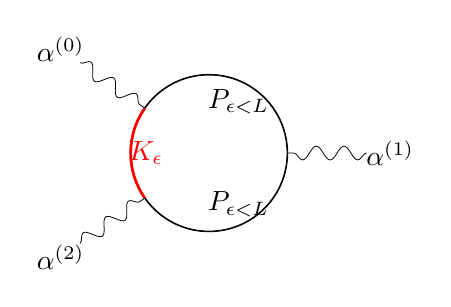
\begin{tikzpicture}[line width=.1mm, scale=1]

%\pgfmathsetmacro{\ex}{0}
%\pgfmathsetmacro{\ey}{1}

%\draw (\ex,\ey) ++(45:.8) arc (45:-45:.8);

		\draw[fill=black] (0,0) circle (1cm);
		%\draw[fill=red] (0,0) arc (145:215:1);
		\draw[fill=white] (0,0) circle (0.99cm);
		\draw[line width=0.35mm,red] ++(145:0.995) arc (145:215:0.995);
		%\draw[red] (0,0) arc (30:60:3);

		\draw[vector](145:2) -- (145:1);
		\node at (145:2.3) {$\alpha^{(0)}$};
			%\node at (145:0.85) {$v_0$};
		\node at (60:0.75) {$P_{\epsilon<L}$};
		\node at (-60:0.75) {$P_{\epsilon<L}$};
		\draw[vector](215:2) -- (215:1cm);
		\node at (215:2.3) {$\alpha^{(2)}$};
			%\node at (215:0.85) {$v_{d}$};
		\node[red] at (180:0.8) {$K_\epsilon$};
		\draw[vector](0:2) -- (0:1);
		\node at (0:2.3) {$\alpha^{(1)}$};
			%\node at (35:0.85) {$v_{\alpha}$};
		%\node at (0:0.8) {$P_{\epsilon<L}$};
		%\node at (270:0.8) {$P_{\epsilon<L}$};
	    	\clip (0,0) circle (1cm);
\end{tikzpicture}
\end{center}
\end{figure}

This gives a holomorphic characterization, and generalization, of the Adler-Bell-Jackiw anomaly for four-dimensional gauge theory.
\end{frame}

\begin{frame}
\frametitle{The holomorphic $\sigma$-model}
The holomorphic $\sigma$-model is a prototypical holomorphic theory. 
Let $X, Y$ be complex manifolds and consider the mapping space:
\ben
{\rm Map}^{hol}(Y,X) = \{f : Y \to X \;\; {\rm holomorphic}\}.
\een
There are a few issues:
\begin{enumerate}
\item
a classical theory involves a shifted symplectic pairing. 
The theory we study is of the form
\ben
T^*[-1] \left({\rm Map}^{hol}(Y,X)\right) .
\een
In degree zero, the fields consist of a map $\gamma : Y \to X$ together with a class $\beta \in \Omega^{d, d-1}(Y , \gamma^* T^{*1,0} X)$. 
The action functional is
\ben
S(\beta,\gamma) = \int_Y \beta \wedge \dbar \gamma .
\een
Notice when we vary $\gamma,\beta$ we obtain $\dbar \gamma = 0 = \dbar \beta$.
\item 
To make this into a BV theory, we must perturb around a fixed holomorphic map;
we look at the formal neighborhood of constant maps ${\rm Map}(Y, X)^{\wedge}_{const}$. 
\end{enumerate}
\end{frame}

\begin{frame}[fragile]
\frametitle{Local-to-global}
Our construction of the holomorphic $\sigma$-model is local-to-global on the target manifold. 
We phrase the theory in the style of {\em formal geometry} due to Gelfand, Kazhdan, Fuks. 
To every $n$-dimensional manifold $X$ (smooth, complex, symplectic, etc..) there exists a universal bundle of coordinates:
\ben
\begin{tikzcd}
\W_n  & \arrow[loop left] X^{coor} \arrow[dd] \arrow[dr] & \\
& & {\rm Fr}_X \arrow[dl] \arrow[ul, "\sigma"', "\simeq", bend right=30] \\
& X & .
\end{tikzcd}
\een
$X^{coor}$ is a principal ${\rm Aut}_n$-bundle together with a transitive action of the Lie algebra of {\em formal vector fields} in $n$-dimensions $\W_n$. 
There is
\ben
\omega^{coor} \in \Omega^1(X^{coor}, \W_n)^{{\rm Aut}_n} \xto{\sigma^*} \Omega^{1}({\rm Fr}_X , \W_n)^{\GL_n}
\een
satisfying the Maurer-Cartan equation $\d \omega^{coor} + \frac{1}{2} [\omega^{coor},\omega^{coor}] = 0$.
\end{frame}

\begin{frame}[fragile]
\frametitle{Gelfand-Kazhdan descent}
Define a category of ``formal vector bundles" on the formal $n$-disk. 
In particular, these are $(\W_n, \GL_n)$-modules. 
For each $X$, there is a functor
\ben
\begin{tikzcd}[row sep = small]
\sV \arrow[r, mapsto] \arrow[d, phantom, "\vin"] & \left({\rm Fr}_X \times^{\GL_n} \sV, \nabla^{coor}\right)  \arrow[d, phantom, "\vin"] \\
{\rm VB}_{\hD^n} \arrow[r,"\desc_X"] \arrow[d, hook] & {\rm VB}^{flat}_{X} \arrow[d,hook] \\
{\rm Mod}_{(\W_n, \GL_n)} \arrow[r] & {\rm Mod}_{D_X} . 
\end{tikzcd}
\een
Moreover, there are ``formal characteristic classes" that live in the Gelfand-Fuks cohomology.
The descent functor determines a transformation of cohomology theories and hence a map of complexes
\ben
{\rm char}_X : \clie^*(\W_n , \GL_n ; \sV) \to \Omega^*(X, \desc_X(\sV)) .
\een

When $\sV = \hO_n$ formal power series, $\desc_X(\hO_n) = J^\infty \sO_X$ equipped with its natural flat connection.
Recover all natural bundles in this way.

\end{frame}

\begin{frame}[fragile]

\frametitle{The formal holomorphic $\sigma$-model}

Consider the formal disk $\hD^n$ as a ringed space whose functions are formal power series $\hO_n$.
\ben
\begin{tikzcd}
Y \arrow[r] & \hD^n \arrow[loop right] & (\W_n,\GL_n) .
\end{tikzcd}
\een

{\bf Key idea:} study the free theory {\em equivariant} for the action of the pair $(\Vect, \GL_n)$.
Get global target $\sigma$-model via descent.

Quantization: holomorphic theory $\implies$ renormalization is simple. 
Obstruction is controlled by an element in Gelfand-Fuks cohomology.

\begin{thm}
There is an obstruction to quantizing the formal holomorphic $\sigma$-model of maps $\CC^d \to \hD^n$ given by the class
\ben
\ch_{d+1}^{\GF} (\hT_n) \in \clie^{d+1}(\W_n , \GL_n; \hOmega^{d+1}_{n,cl}) .
\een
\end{thm}

Under characteristic map, this returns the ordinary Chern class. 
Determines an {\em $L_\infty$-extension}
\ben
0 \to \hOmega^{d+1}_{n,cl} \to \TVectd \to \W_n \to 0 .
\een
\end{frame}

\begin{frame}[fragile]
\frametitle{Extended descent}
Given any trivialization $\alpha$ of $\ch_{d+1}(T_X)$ we can lift the structure of the coordinate bundle. 
\ben
\begin{tikzcd}
\TVectd \arrow[d] & \arrow[loop left] \Tilde{X}^{coor}_{\alpha} \arrow[d, dotted] \arrow[dr, dotted] & &   \\ 
\W_n & \arrow[loop left] X^{coor} \arrow[dd] \arrow[dr] & ({\rm Fr}_X, \Tilde{\omega}_{\alpha}^{coor})\arrow[d] &   \Tilde{\omega}^{coor}_{\alpha} \in \oplus_{p\geq 1} \Omega^p({\rm Fr}_X , \TVectd)  \\
& & ({\rm Fr}_X, \omega^{coor}) \arrow[dl] &  \d \Tilde{\omega}^{coor}_{\alpha} + \sum_{k \geq 2} \ell_k(\Tilde{\omega}^{coor}_{\alpha}) = 0 \\
& X & &
\end{tikzcd}
\een
Descent functor
\ben
\Tilde{\desc}_{X,\alpha} : {\rm Mod}_{(\TVectd, \GL_n)} \to {\rm Mod}_{D_X} .
\een
Theorem implies quantization is equivariant for $(\TVectd, \GL_n)$. 
This says that for any trivialization $\alpha$ we obtain a global quantization. 

\end{frame}

\begin{frame}
\frametitle{Main result}
Explicit GF calculation shows there is a unique $(\TVectd, \GL_n)$-quantization for the formal theory.
Extended descent implies the following main result.

\begin{thm} Suppose $\ch_{d+1}(T_X) = 0$.
Then, the space of quantizations (respecting certain natural symmetries) of the holomorphic $\sigma$-model of maps $\CC^d \to X$ is a torsor for the abelian group $H^{d}(X , \Omega^{d+1,hol}_X)$. 
\end{thm}

\begin{itemize}
\item Quantizations exist on other source manifolds: affine manifolds, abelian varieties, Hopf manifolds $Y = \CC^d \setminus \{0\} / q^\ZZ \cong S^{2d-1} \times S^1$. 
\item Local calculation of the index produces elliptic $\Gamma$-functions.
This agrees with the partition function for supersymmetric theories in dimensions $2,4,6$. 
For a general target, this should produced refined invariants generalizing the Witten genus in complex dimension one.
\end{itemize}
\end{frame}

\begin{frame}[fragile]

\frametitle{Relation to deformation quantization}

Immediate corollary: obtain the following deformation quantization for ''sphere algebras". 
Theory on 
\ben
\begin{tikzcd}
\CC^{d} \setminus \{0\} \arrow[d,"\pi"'] \arrow[r, "\cong"] & \RR_{>0} \times S^{2d-1} \\
\RR_{>0} . 
\end{tikzcd}
\een
Reduction along the sphere:
\ben
\begin{tikzcd}
\pi_*\left({\rm Holomorphic\;}\sigma {\rm -model} \; \CC^d \setminus \{0\} \to X\right) \arrow[d, equals] \\
{\rm One \; dimensional\;} \sigma {\rm -model} \; \RR_{>0} \to T^* {\rm Map}^{alg}(S^{2d-1}, X) .
\end{tikzcd}
\een
Sphere mapping space is really a derived algebraic version.
There is a dg algebra $A_d$ with $A_d^0 \hookrightarrow C^\infty(S^{2d-1})$ densely and
\ben
A_d \hookrightarrow \Omega^{0,*}(\CC^d \setminus \{0\})
\een
which is dense in cohomology. 
When $d=1$, $A_1 = \CC[z,z^{-1}]$ and we get algebraic loop space.

\end{frame}

\begin{frame}[fragile]

\frametitle{Observables}

BV quantization produces a (sheaf of) factorization algebras on $\CC^{d}$. 
In the one-dimensional reduction, restricts to a factorization algebra on $\RR_{>0} \rightsquigarrow$ dg associative algebra.
When $\ch_{d+1}(T_X) = 0$ we get a deformation quantization = "differential operators on the sphere mapping space". 
\ben
\begin{tikzcd}
\sO_\hbar \left(T^*{\rm Map}(S^{2d-1}, X)\right) \ar[d,"\hbar \to 0"] \ar[r,equals]& : D_{\hbar}\left({\rm Map}(S^{2d-1}, X)\right) \\
\sO \left(T^*{\rm Map}(S^{2d-1}, X)\right) .
\end{tikzcd}
\een
The state space $\sV_X$ is equal to the observables supported on the disk in $\CC^d$. 
Factorization product endows $\sV_X$ with the structure of a dg module over $D_{\hbar}({\rm Map}(S^{2d-1}, X))$. 
It is equal to the ``vacuum" module
\ben
\sV_X = D_\hbar \tensor_{D_{\hbar,+}} \CC[[\hbar]] .
\een
Where $D_{\hbar,+} \subset D_\hbar$ is a maximal commutative subalgebra of ''positive modes". 
This plays the role of the Hilbert space in quantum mechanics.
\end{frame}

\begin{frame}
\frametitle{Conclusions and outlook}

\begin{itemize}
\item Have not discussed much about "source symmetries" of the holomorphic $\sigma$-model.
Big part of my thesis was to characterize symmetries by holomorphic gauge transformations and by holomorphic diffeomorphisms. 
Lead to higher dimensional Kac-Moody algebras and Virasoro algebras, respectively. 
\item In particular, there is a dg Lie algebra central extension of holomorphic vector fields on punctured affine space that embeds inside of $D_{\hbar}$. 
This central extension is parametrized by a higher dimensional version of ''central charge" in CFT. 
\end{itemize}
\end{frame}

\end{document}